\documentclass[11pt,a4paper]{article}

% ============================================================
% PACKAGES
% ============================================================
\usepackage[utf8]{inputenc}
\usepackage[T1]{fontenc}
\usepackage{lmodern}
\usepackage[margin=1in]{geometry}
\usepackage{graphicx}
\usepackage{booktabs}
\usepackage{longtable}
\usepackage{array}
\usepackage{tabularx}
\usepackage{multirow}
\usepackage{hyperref}
\usepackage{xcolor}
\usepackage{listings}
\usepackage{enumitem}
\usepackage{tikz}
\usetikzlibrary{shapes.geometric, arrows.meta, positioning, fit, calc}
\usepackage{float}
\usepackage{caption}
\usepackage{amsmath}
\usepackage{cite}

\hypersetup{
    colorlinks=true,
    linkcolor=blue!70!black,
    citecolor=green!50!black,
    urlcolor=blue!60!black
}

\lstset{
    basicstyle=\ttfamily\small,
    breaklines=true,
    frame=single,
    backgroundcolor=\color{gray!10},
    keywordstyle=\color{blue!70!black}\bfseries,
    commentstyle=\color{green!50!black},
    stringstyle=\color{red!60!black},
}

% ============================================================
% TITLE
% ============================================================
\begin{document}

\begin{center}
    {\LARGE\bfseries Phase 1: Literature Review, Research Gaps, Proposal \& Baseline} \\[0.5em]
    {\Large AI4015 -- Agentic Artificial Intelligence} \\[1em]
    {\large\bfseries Project Code: G1} \\[0.3em]
    {\large\bfseries Project Title: SpecLoop -- Formal Specification-Driven Verification Feedback Pipeline for LLM Coding Agents} \\[1em]
    
    \begin{tabular}{lll}
        \textbf{Name} & \textbf{Roll Number} & \textbf{Role} \\
        \midrule
        Syed Muhammad Hassan & 23i-0519 & Group Head \\
        Abdul Majeed & 23p-3038 & Member \\
    \end{tabular}
    
    \vspace{1em}
    {\large Supervisor: Muhammad Sajjad} \\[0.3em]
    {\large Date: October 2026}
\end{center}

\vspace{1em}
\hrule
\vspace{1em}

\tableofcontents
\newpage

% ============================================================
% DELIVERABLE A: LITERATURE REVIEW & RESEARCH GAPS
% ============================================================
\section*{Deliverable A: Literature Review \& Research Gaps}
\addcontentsline{toc}{section}{Deliverable A: Literature Review \& Research Gaps}

% ============================================================
\section{Paper Selection}
% ============================================================

We identified and critically studied 10 research papers from 2025--2026 that are directly related to formal specification-driven development with AI coding agents. All papers are published in peer-reviewed venues including ICLR, ICML, NeurIPS, ICSE, OOPSLA, and TMLR. Paper 1 is the selected base paper.

% ============================================================
\section{Base Paper}
% ============================================================

\textbf{Base Paper:} Sun et al., ``VERINA: Benchmarking LLMs on Verifiable Code Generation,'' \textit{International Conference on Learning Representations (ICLR)}, 2026 \cite{verina2026}.

\textbf{Proof of Ranking:} ICLR is ranked \textbf{A*} by the CORE Conference Rankings Portal (portal.core.edu.au, ID: 2273). This satisfies the A*/A requirement.

\textbf{Why Selected:} VERINA is the most directly relevant benchmark to our project. It defines the task of verifiable code generation---requiring LLMs to jointly produce code, formal specifications, and machine-checkable proofs---which is precisely the problem domain our verification-feedback pipeline targets. Its modular evaluation framework (evaluating code, spec, and proof independently or jointly) provides the evaluation template our cross-model and cross-language comparison builds upon. Critically, VERINA uses Lean 4 only and explicitly leaves Dafny, Verus, and contract-language support to future work, creating the research gap our project fills.

\subsection{Base Paper Analysis}

\textbf{Problem:} Existing code-generation benchmarks rely on finite test suites that leave subtle bugs undetected. VERINA addresses the need for a benchmark that evaluates whether LLMs can generate provably correct code with machine-checkable guarantees.

\textbf{Method:} VERINA provides 189 manually curated coding tasks in Lean 4, each with a problem description, reference implementation, formal specification, and extensive test suite. It evaluates LLMs on three subtasks independently: code generation, specification writing, and proof synthesis.

\textbf{Dataset:} 189 tasks in Lean 4, spanning difficulty levels from basic arithmetic to algorithm design.

\textbf{Key Results:} Top models (e.g., OpenAI o3) achieve 72.6\% code correctness, 52.3\% specification soundness, but only 4.9\% proof generation success rate. This reveals a massive gap between code generation and formal proof capabilities.

\textbf{Limitations (Author-Stated):}
\begin{itemize}[noitemsep]
    \item Only Lean 4 is supported; Dafny, Verus, F*, and mainstream contract libraries are not evaluated.
    \item No feedback loop---LLMs generate code in a single shot without iterative repair.
    \item No comparison between verification languages under the same evaluation conditions.
\end{itemize}

\textbf{Limitations (Our Analysis):}
\begin{itemize}[noitemsep]
    \item No testing-only baseline---cannot quantify the added value of formal verification over tests alone.
    \item Models are evaluated at a single snapshot; no study of how verifier feedback improves correctness over iterations.
    \item The benchmark does not cover contract-based specifications in mainstream languages (Python, Rust), limiting practical applicability.
\end{itemize}

\textbf{How Our Project Builds On It:} We adopt VERINA's modular evaluation methodology but extend it to: (a) compare Dafny and Python/iContract as specification languages, (b) add a verification-feedback loop with iterative repair, and (c) include a testing-only baseline for controlled comparison.

% ============================================================
\section{Critical Paper Summaries}
% ============================================================

\subsection{Paper 1 (Base Paper): VERINA -- Benchmarking LLMs on Verifiable Code Generation}
\textit{Sun et al., ICLR 2026} \cite{verina2026}

VERINA introduces a modular benchmark of 189 Lean 4 tasks for evaluating LLMs on verifiable code generation, requiring models to produce code, specifications, and machine-checkable proofs. The benchmark enables independent evaluation of each subtask. Testing frontier models, the authors find that while top models achieve 72.6\% code correctness, proof generation rates are extremely low (4.9\% for o3). The modular design reveals that specification quality is a key bottleneck---models that write better specs also produce more verifiable code. \textbf{Limitations:} Single-language (Lean 4) focus; no iterative feedback; no testing-only baseline; no comparison of verification languages. \textbf{Relevance:} Directly defines the evaluation framework we extend with multi-language support and a feedback loop.

\subsection{Paper 2: AlphaVerus -- Bootstrapping Formally Verified Code Generation through Self-Improving Translation and Treefinement}
\textit{Aggarwal et al., ICML 2025} \cite{alphaVerus2025}

AlphaVerus presents a self-improving framework for generating formally verified Rust code using the Verus verifier. It uses a three-phase pipeline: (1) translating programs from Dafny to Verus using an LLM, (2) refining candidates via a novel tree-search algorithm (Treefinement) guided by verifier feedback, and (3) filtering out misaligned specifications. Applied to LLaMA-3.1-70B without fine-tuning, it achieves state-of-the-art results on HumanEval and MBPP translated to Verus. \textbf{Limitations:} Relies on Dafny$\to$Verus translation rather than direct generation; no comparison with contract-based approaches in mainstream languages; tree search is computationally expensive; no combined testing+verification feedback. \textbf{Relevance:} Demonstrates that verifier feedback loops improve code correctness, validating our core hypothesis. Our system differs by comparing languages and combining testing with verification.

\subsection{Paper 3: CLEVER -- A Curated Lean Verified Code Generation Benchmark}
\textit{NeurIPS 2025, Datasets \& Benchmarks Track} \cite{clever2025}

CLEVER provides 161 hand-curated problems requiring LLMs to generate both Lean 4 implementations and machine-checkable proofs, validated by Lean's native type checker. Unlike benchmarks that accept passing test suites, CLEVER demands mathematical proof of correctness. Evaluations show that current frontier models struggle significantly with full verification, highlighting the gap between code generation and formal reasoning. \textbf{Limitations:} Lean 4 only; no iterative feedback mechanism; no cross-language comparison; limited to specification generation + proof, not the full development loop. \textbf{Relevance:} Provides an additional verification benchmark demonstrating that formal proof remains a bottleneck, motivating our approach of combining verifier feedback with runtime tests.

\subsection{Paper 4: SpecGen -- Automated Generation of Formal Program Specifications via LLMs}
\textit{Ma et al., ICSE 2025} \cite{specgen2025}

SpecGen combines LLM-driven conversational specification generation with a mutation-based selection strategy. In a two-phase pipeline, it first uses few-shot prompting with verification error feedback to iteratively refine specifications, then applies four mutation operators (logical, comparative, predicative, arithmetic) to generate variants and selects verifiable ones. Evaluated on SV-COMP Java benchmarks, it generates verifiable specifications for 279/385 programs, outperforming Daikon and Houdini. \textbf{Limitations:} Focuses on specification generation, not code generation; Java only; does not study how generated specifications help guide code repair; mutation operators are domain-specific. \textbf{Relevance:} Demonstrates that LLMs can generate formal specifications when guided by verifier feedback, which our pipeline leverages---we use pre-given specifications and study whether LLMs can generate code satisfying them.

\subsection{Paper 5: AutoVerus -- Automated Proof Generation for Rust Code}
\textit{OOPSLA 2025} \cite{autoverus2025}

AutoVerus employs a network of collaborative LLM agents to generate formal proofs for Rust code using the Verus verifier. The three-phase pipeline mimics human proof-writing: preliminary generation, refinement using generic tips, and debugging driven by symbolic verification errors. Evaluated on Verus-Bench (150 tasks), it automatically proves over 90\% of tasks, with most solutions found within 3 LLM calls. \textbf{Limitations:} Verus/Rust only; proof generation focus (not code+proof); multi-agent orchestration adds complexity; no comparison with simpler single-agent approaches or with testing-only pipelines. \textbf{Relevance:} Validates multi-step verifier-feedback loops for proof synthesis. Our work differs by targeting code generation (not just proofs) and comparing specification languages.

\subsection{Paper 6: Towards Neural Synthesis for SMT-Assisted Proof-Oriented Programming}
\textit{Chakraborty et al., ICSE 2025} \cite{fstar2025}

This paper curates a large-scale dataset of F* programs ($\sim$600K--940K lines) from production systems (Windows, Linux, HACL*) and uses it to benchmark LLM-driven proof synthesis. It treats proof construction as type-directed synthesis, interfacing with the F* compiler. Key finding: smaller fine-tuned models (e.g., Phi-2) match GPT-4 on specialized proof tasks, and type-based retrieval-augmented generation significantly boosts accuracy. \textbf{Limitations:} F* only; requires fine-tuning for best results; production code complexity limits reproducibility; no comparison with contract-based or Dafny approaches. \textbf{Relevance:} Shows that different verification ecosystems (F*, Dafny, Verus) have distinct characteristics affecting LLM performance, motivating our cross-language comparison.

\subsection{Paper 7: DafnyBench -- Benchmarking AI for Formal Software Verification}
\textit{TMLR 2025} \cite{dafnybench2025}

DafnyBench provides 750+ verified Dafny programs ($\sim$53K lines) for evaluating LLMs on annotation generation---specifically loop invariants, specifications, and hints needed for Dafny verification. GPT-4 and Claude 3 achieve $\sim$68\% success rate with iterative error feedback. The study shows that LLM performance improves with verifier error messages but drops as required annotation volume scales up. \textbf{Limitations:} Focuses on hint/annotation generation, not full code generation; Dafny only; no comparison with testing-only approaches; no systematic study of different feedback strategies. \textbf{Relevance:} Directly relevant as our Dafny benchmark source and validates that verifier feedback improves LLM output. We extend this to full code generation with specification-driven feedback.

\subsection{Paper 8: FVAPPS -- Proving the Coding Interview}
\textit{Dougherty et al., LLM4Code Workshop at ICSE 2025} \cite{fvapps2025}

FVAPPS is the largest formal verification benchmark with 4,715 samples (1,083 curated) in Lean 4, generalizing traditional unit tests into formal theorems. It evaluates whether LLMs can not only write code but prove its correctness. Baseline evaluations show Claude Sonnet proves 30\% and Gemini proves 18\% of theorems, highlighting substantial room for improvement. \textbf{Limitations:} Lean 4 only; no iterative feedback; workshop paper with limited experimental depth; no cross-model systematic comparison; benchmark quality varies across non-curated samples. \textbf{Relevance:} Provides a large-scale benchmark and baseline numbers showing the difficulty of formal proof generation, contextualizing our work's focus on combining testing with verification.

\subsection{Paper 9: Towards Understanding the Characteristics of Code Generation Errors Made by LLMs}
\textit{Wang et al., ICSE 2025} \cite{codeerrors2025}

This empirical study analyzes code generation errors across six LLMs (CodeGen, InCoder, GPT-3.5, GPT-4) on HumanEval, building a comprehensive taxonomy of semantic and syntactic errors. Key finding: LLMs rarely make simple syntax errors---instead, they produce multi-line logic and structural errors that are difficult to detect with tests alone. Error profiles shift dramatically with task complexity. \textbf{Limitations:} Descriptive study with no automated repair mechanism; Python only; test-based evaluation only; no formal verification analysis of error types. \textbf{Relevance:} Provides empirical evidence that tests miss subtle semantic errors, directly motivating our use of formal verification to catch errors that testing cannot.

\subsection{Paper 10: TOGLL -- Correct and Strong Test Oracle Generation with LLMs}
\textit{ICSE 2025} \cite{togll2025}

TOGLL fine-tunes seven code LLMs on 110 Java projects to generate correct and strong test oracles (assertions). The optimized configuration produces 3.8x more correct assertions than TOGA, detects 1,023 unique mutants missed by EvoSuite, and significantly outperforms baselines on Defects4J real-world bugs. \textbf{Limitations:} Java only; requires fine-tuning; test oracle generation only---does not integrate formal verification; generated tests may still miss specification violations that verification would catch. \textbf{Relevance:} Demonstrates that LLM-generated tests can be strong but not complete. Our project complements this by showing that formal verification catches errors that even strong LLM-generated tests miss.


% ============================================================
\section{Cross-Paper Comparison Table}
% ============================================================

\begin{table}[H]
\centering
\caption{Cross-Paper Comparison (Base paper marked with *)}
\label{tab:comparison}
\scriptsize
\begin{tabularx}{\textwidth}{|c|p{2cm}|c|p{1.8cm}|p{2cm}|p{1.5cm}|p{1.5cm}|p{2cm}|}
\hline
\textbf{\#} & \textbf{Title} & \textbf{Year/Venue} & \textbf{Dataset} & \textbf{Method} & \textbf{Metrics} & \textbf{Key Results} & \textbf{Limitations / Gap} \\
\hline
1* & VERINA \cite{verina2026} & 2026 ICLR & 189 Lean 4 tasks & Modular eval: code + spec + proof & Correctness, soundness, proof rate & 72.6\% code, 4.9\% proof & Lean only; no feedback loop; no testing baseline \\
\hline
2 & AlphaVerus \cite{alphaVerus2025} & 2025 ICML & HumanEval, MBPP (Verus) & Translation + Treefinement + filter & Verified rate & SOTA on Verus benchmarks & Verus only; no cross-language; expensive search \\
\hline
3 & CLEVER \cite{clever2025} & 2025 NeurIPS & 161 Lean 4 problems & End-to-end verified generation & Proof success rate & Models struggle with proofs & Lean only; no feedback; no cross-lang \\
\hline
4 & SpecGen \cite{specgen2025} & 2025 ICSE & SV-COMP Java & Conversational + mutation & Verifiable specs & 279/385 verified & Spec-gen only; Java; no code repair \\
\hline
5 & AutoVerus \cite{autoverus2025} & 2025 OOPSLA & Verus-Bench 150 tasks & Multi-agent proof gen & Proof rate, time & 90\%+ proved & Verus only; proof-only; complex \\
\hline
6 & F* Neural Syn. \cite{fstar2025} & 2025 ICSE & 600K lines F* & Fine-tuned + RAG & Synthesis success & Phi-2 matches GPT-4 & F* only; needs fine-tuning \\
\hline
7 & DafnyBench \cite{dafnybench2025} & 2025 TMLR & 750+ Dafny programs & Hint generation + feedback & Annotation success & 68\% with feedback & Annotations only; no full code gen \\
\hline
8 & FVAPPS \cite{fvapps2025} & 2025 ICSE-W & 4,715 Lean 4 & Formal theorem proving & Proof rate & 30\% (Sonnet) & Lean only; no feedback loop \\
\hline
9 & Code Errors \cite{codeerrors2025} & 2025 ICSE & HumanEval & Error taxonomy & Error types, rates & Multi-line semantic errors & Descriptive; no repair; tests only \\
\hline
10 & TOGLL \cite{togll2025} & 2025 ICSE & 110 Java projects & Fine-tuned oracle gen & Oracle correctness, mutants & 3.8x better than TOGA & Java; tests only; no verification \\
\hline
\end{tabularx}
\end{table}


% ============================================================
\section{Research Gap Synthesis}
% ============================================================

Based on our analysis of the 10 reviewed papers, we identified the following three strong, evidence-based research gaps:

\begin{table}[H]
\centering
\caption{Research Gaps}
\label{tab:gaps}
\small
\begin{tabularx}{\textwidth}{|c|X|X|X|}
\hline
\textbf{Gap} & \textbf{Supporting Evidence} & \textbf{Proposed Approach} & \textbf{Measurement} \\
\hline
\textbf{Gap 1:} No controlled comparison of contract-based specification languages under a unified agent feedback loop. & 
VERINA \cite{verina2026} uses Lean only; AlphaVerus \cite{alphaVerus2025} uses Verus only; DafnyBench \cite{dafnybench2025} uses Dafny only; F* Neural Synthesis \cite{fstar2025} uses F* only. No paper compares languages under identical agent and evaluation conditions. &
Implement Dafny and Python/iContract backends in a single pipeline with identical prompts, tasks, and feedback loops. Evaluate the same LLMs on equivalent tasks in both languages. &
Compare verification rate, test pass rate, correctness rate, and average repair iterations across languages for the same model and tasks. Statistical significance via paired tests. \\
\hline
\textbf{Gap 2:} Existing repair loops use verifier errors for feedback but treat testing as a separate scoring mechanism, not as a complementary feedback signal. & 
AlphaVerus \cite{alphaVerus2025} and AutoVerus \cite{autoverus2025} use only verifier errors; DafnyBench \cite{dafnybench2025} shows feedback helps but tests are used only for evaluation; Code Errors \cite{codeerrors2025} shows tests miss semantic bugs; TOGLL \cite{togll2025} generates tests but doesn't combine with verification. &
Implement a combined agent that sends both verifier errors AND test failures as structured feedback to the LLM, compared against verifier-only and testing-only agents. &
Compare correctness rate of combined agent vs. verifier-only vs. testing-only agents. Measure how many errors are caught exclusively by tests vs. exclusively by verification. \\
\hline
\textbf{Gap 3:} Cross-model evaluations are done in single-shot mode without a testing-only agent baseline, making it impossible to quantify the marginal benefit of formal verification. &
VERINA \cite{verina2026} evaluates models in single-shot; CLEVER \cite{clever2025} provides no iterative baseline; FVAPPS \cite{fvapps2025} lacks systematic cross-model comparison; no paper provides a testing-only agent as a controlled baseline. &
Evaluate multiple LLMs (GPT-4o, Claude, etc.) across all four agent modes (single-shot, testing-only, verifier-feedback, combined) on the same benchmark tasks. &
Measure the correctness gain ($\Delta$) from testing-only to verifier-feedback and combined modes, per model. Compute cost-effectiveness as correctness gain per API dollar. \\
\hline
\end{tabularx}
\end{table}


\newpage
% ============================================================
% DELIVERABLE B: PROJECT PROPOSAL
% ============================================================
\section*{Deliverable B: Project Proposal}
\addcontentsline{toc}{section}{Deliverable B: Project Proposal}

% ============================================================
\section{Project Title and Selected Seed}
% ============================================================

\textbf{Selected Seed:} G1 -- Formal Specification-Driven Development with AI Coding Agents

\textbf{Project Title:} \textit{SpecLoop: Formal Specification-Driven Verification Feedback Pipeline for LLM Coding Agents}

% ============================================================
\section{Problem Statement and Motivation}
% ============================================================

\textbf{Problem:} LLM-based coding agents generate code impressively but produce subtle semantic errors---multi-line logic bugs, edge-case failures, and specification violations---that evade finite test suites \cite{codeerrors2025}. In domains requiring correctness guarantees (finance, healthcare, aerospace), this limits adoption.

\textbf{Target Users:} Software development teams in safety-critical domains; researchers studying LLM code generation reliability; organizations evaluating coding agent deployment.

\textbf{Current Limitations:} Existing approaches either (a) evaluate in single-shot mode without feedback loops \cite{verina2026, clever2025}, (b) use only one verification language per study \cite{alphaVerus2025, autoverus2025, dafnybench2025}, or (c) treat testing and formal verification as separate concerns \cite{togll2025, codeerrors2025}.

\textbf{Why It Matters:} A controlled comparison of specification languages and feedback strategies, with a testing-only baseline, would provide actionable evidence for practitioners choosing verification tools and for researchers designing coding agent architectures.

% ============================================================
\section{Base Paper and Research Gaps}
% ============================================================

VERINA \cite{verina2026} (ICLR 2026, A*-ranked) is our base paper. It provides the definitive benchmark for verifiable code generation, evaluating frontier LLMs on code, specification, and proof generation in Lean 4. Our project addresses its three main limitations:

\begin{enumerate}[noitemsep]
    \item \textbf{Gap 1:} VERINA supports only Lean 4. We compare Dafny and Python/iContract under identical conditions.
    \item \textbf{Gap 2:} VERINA uses single-shot evaluation. We add a verification-feedback loop combined with testing.
    \item \textbf{Gap 3:} VERINA provides no testing-only baseline. We include all four agent modes for controlled ablation.
\end{enumerate}

% ============================================================
\section{Target Product or System}
% ============================================================

The end-of-semester deliverable is \textbf{SpecLoop}, an open-source verification-feedback pipeline comprising:

\begin{enumerate}[noitemsep]
    \item A \textbf{multi-backend verification engine} supporting Dafny and Python/iContract+CrossHair.
    \item A \textbf{specification integrity guard} that detects and rejects LLM attempts to weaken or remove specifications.
    \item \textbf{Four agent modes} (single-shot, testing-only, verifier-feedback, combined) for controlled ablation.
    \item A \textbf{benchmark suite} with tasks in both Dafny and Python contract forms.
    \item An \textbf{evaluation framework} producing cross-model, cross-language, cross-mode comparison tables.
    \item A \textbf{CLI tool} for running experiments end-to-end.
\end{enumerate}

% ============================================================
\section{Agentic Justification}
% ============================================================

This problem \textit{requires} agentic behavior and cannot be solved by a deterministic workflow, a single LLM call, or a simple RAG pipeline:

\begin{itemize}[noitemsep]
    \item \textbf{Iterative reasoning under feedback:} The agent must interpret verifier error messages, reason about why its code violates the specification, and generate targeted repairs. This requires multi-step reasoning conditioned on evolving state---not a single call.
    \item \textbf{Tool use:} The agent must invoke external tools (Dafny verifier, CrossHair analyzer, test runners) and parse their structured output, which varies per attempt.
    \item \textbf{Adaptive strategy:} When verification fails, the nature of the failure determines the repair strategy. Specification violations require different fixes than runtime test failures. The agent must adapt its approach based on feedback type---a planning capability.
    \item \textbf{Stateful multi-turn interaction:} The agent maintains context across multiple generation-verification cycles, remembering previous attempts and their failures to avoid repeating the same errors.
    \item \textbf{Why not RAG?} Retrieval alone cannot solve this---the problem is not finding information but reasoning over formal verification constraints and generating correct code. The feedback loop is the core agentic mechanism.
\end{itemize}

% ============================================================
\section{Goals and Success Criteria}
% ============================================================

\subsection{Development Objectives}
\begin{enumerate}[noitemsep]
    \item Implement Dafny and Python/iContract verification backends with specification integrity guards.
    \item Build four agent modes with a unified pipeline architecture.
    \item Create a benchmark suite of $\geq$20 tasks per language.
    \item Integrate $\geq$2 LLM providers (OpenAI, Anthropic).
    \item Produce automated evaluation reports with comparison tables.
\end{enumerate}

\subsection{Research Objectives and Success Criteria}

\begin{table}[H]
\centering
\small
\begin{tabularx}{\textwidth}{|c|X|X|}
\hline
\textbf{Gap} & \textbf{Research Objective} & \textbf{Success Criterion} \\
\hline
Gap 1 & Quantify verification-rate difference between Dafny and Python/iContract & Statistically significant difference observed (paired t-test, $p < 0.05$) OR evidence of equivalence \\
\hline
Gap 2 & Show combined (verifier+test) feedback outperforms either alone & Combined agent correctness rate $\geq 5\%$ higher than verifier-only and testing-only agents \\
\hline
Gap 3 & Measure correctness gain of verification-feedback over testing-only baseline, across models & Verifier-feedback agent achieves $\geq 10\%$ higher correctness than testing-only baseline on $\geq 1$ model \\
\hline
\end{tabularx}
\end{table}

% ============================================================
\section{Data / Environment / Source}
% ============================================================

\begin{itemize}[noitemsep]
    \item \textbf{Dafny Benchmark:} Custom-created tasks with formal specifications (preconditions, postconditions, loop invariants). Initial set of 5 tasks provided; will expand to 20+ using MBPP-DFY-50 benchmark \cite{dafnybench2025} and DafnyBench \cite{dafnybench2025} problems.
    \item \textbf{Python Contract Benchmark:} Custom tasks with iContract decorators. Initial set of 2 tasks provided; will expand to 20+ with equivalent problems.
    \item \textbf{LLM APIs:} OpenAI API (GPT-4o) and Anthropic API (Claude Sonnet). Mock provider for development.
    \item \textbf{Verification Tools:} Dafny 4.x (with Z3 solver); CrossHair (Python symbolic executor); iContract (runtime contracts).
    \item \textbf{Status:} Data pipeline is confirmed and working. 7 benchmark tasks loaded, mock evaluation runs end-to-end.
\end{itemize}

% ============================================================
\section{System Architecture}
% ============================================================

The SpecLoop system comprises five major components:

\begin{enumerate}[noitemsep]
    \item \textbf{Benchmark Loader:} Reads task specifications from JSON files, supporting both Dafny and Python/iContract formats.
    \item \textbf{LLM Provider Layer:} Abstracts OpenAI and Anthropic APIs behind a common interface. A Mock provider enables testing without API calls.
    \item \textbf{Agent Layer:} Four agent implementations (SingleShot, TestingOnly, VerifierFeedback, Combined) sharing the same prompt templates and code-extraction logic.
    \item \textbf{Verification Backends:} DafnyBackend (calls \texttt{dafny verify} and \texttt{dafny run}) and PythonContractBackend (calls CrossHair and runs iContract-decorated code). Both include specification integrity guards.
    \item \textbf{Evaluator:} Aggregates PipelineResult objects and computes cross-model/cross-language/cross-mode metrics.
\end{enumerate}

% ============================================================
\section{Methodology / Architecture Diagram}
% ============================================================

\begin{figure}[H]
\centering
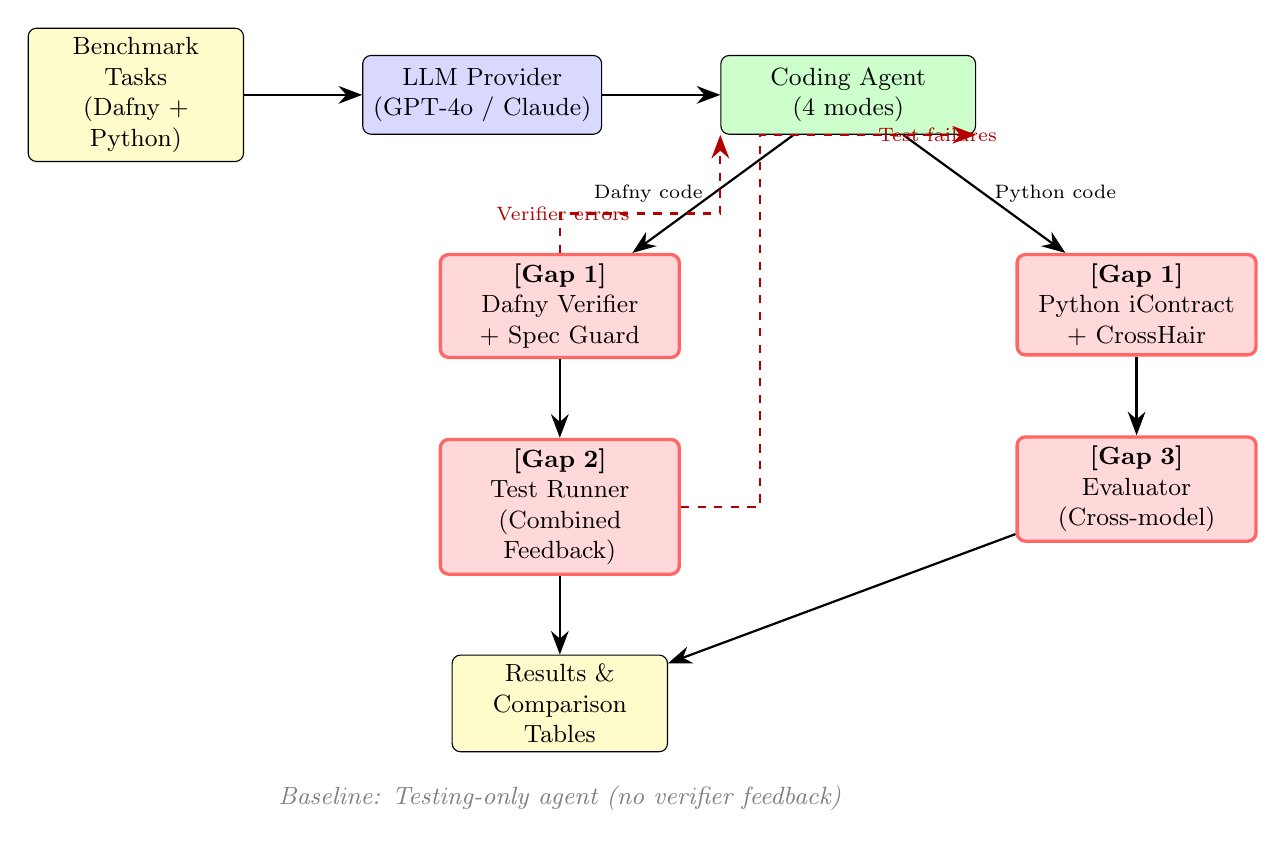
\begin{tikzpicture}[
    node distance=1cm and 1.5cm,
    block/.style={rectangle, draw, fill=blue!15, text width=2.8cm, minimum height=1cm, align=center, rounded corners=3pt, font=\small},
    agent/.style={rectangle, draw, fill=green!20, text width=3cm, minimum height=1cm, align=center, rounded corners=3pt, font=\small},
    backend/.style={rectangle, draw, fill=orange!20, text width=2.8cm, minimum height=1cm, align=center, rounded corners=3pt, font=\small},
    data/.style={rectangle, draw, fill=yellow!20, text width=2.5cm, minimum height=0.8cm, align=center, rounded corners=3pt, font=\small},
    gap/.style={fill=red!15, draw=red!60, very thick},
    arrow/.style={-{Stealth[length=3mm]}, thick},
    feedback/.style={-{Stealth[length=3mm]}, thick, dashed, red!70!black},
]

% Benchmark
\node[data] (bench) {Benchmark Tasks\\(Dafny + Python)};

% Provider
\node[block, right=1.5cm of bench] (provider) {LLM Provider\\(GPT-4o / Claude)};

% Agent
\node[agent, right=1.5cm of provider] (agent) {Coding Agent\\(4 modes)};

% Backends
\node[backend, below left=1.5cm and 0.5cm of agent, gap] (dafny) {\textbf{[Gap 1]}\\Dafny Verifier\\+ Spec Guard};
\node[backend, below right=1.5cm and 0.5cm of agent, gap] (python) {\textbf{[Gap 1]}\\Python iContract\\+ CrossHair};

% Test runner
\node[backend, below=1cm of dafny, gap] (tests) {\textbf{[Gap 2]}\\Test Runner\\(Combined Feedback)};

% Evaluator
\node[block, below=1cm of python, gap] (eval) {\textbf{[Gap 3]}\\Evaluator\\(Cross-model)};

% Results
\node[data, below=1cm of tests] (results) {Results \&\\Comparison Tables};

% Arrows
\draw[arrow] (bench) -- (provider);
\draw[arrow] (provider) -- (agent);
\draw[arrow] (agent) -- (dafny) node[midway, left, font=\scriptsize] {Dafny code};
\draw[arrow] (agent) -- (python) node[midway, right, font=\scriptsize] {Python code};
\draw[arrow] (dafny) -- (tests);
\draw[arrow] (python) -- (eval);
\draw[arrow] (tests) -- (results);
\draw[arrow] (eval) -- (results);

% Feedback loops
\draw[feedback] (dafny.north) -- ++(0,0.5) -| (agent.south west) node[near start, left, font=\scriptsize, text=red!70!black] {Verifier errors};
\draw[feedback] (tests.east) -- ++(1,0) |- (agent.south east) node[near end, right, font=\scriptsize, text=red!70!black] {Test failures};

% Baseline marker
\node[below=0.3cm of results, font=\small\itshape, text=gray] {Baseline: Testing-only agent (no verifier feedback)};

\end{tikzpicture}
\caption{SpecLoop system architecture. Red-bordered components mark where each research gap is addressed. Dashed arrows show the verification-feedback loop. The baseline (testing-only agent) omits the verifier feedback path.}
\label{fig:architecture}
\end{figure}


% ============================================================
\section{Baseline}
% ============================================================

Our primary baseline is the \textbf{testing-only agent}, which:
\begin{itemize}[noitemsep]
    \item Generates code using the same LLM and prompts as the proposed system.
    \item Receives feedback only from runtime test results (pass/fail + error messages).
    \item Does NOT receive formal verification feedback.
    \item Iterates for the same maximum number of attempts (5).
\end{itemize}

This isolates the contribution of formal verification feedback. Additionally:
\begin{itemize}[noitemsep]
    \item \textbf{Single-shot agent:} No feedback at all (ablation control).
    \item \textbf{VERINA baseline:} We compare against VERINA's reported single-shot numbers for context.
\end{itemize}

% ============================================================
\section{Research Questions and Hypotheses}
% ============================================================

\begin{table}[H]
\centering
\small
\begin{tabularx}{\textwidth}{|c|X|X|}
\hline
\textbf{Gap} & \textbf{Research Question} & \textbf{Hypothesis} \\
\hline
Gap 1 & Does the choice of specification language (Dafny vs. Python/iContract) significantly affect the correctness rate of LLM-generated code under the same feedback loop? & Dafny's stronger type system and built-in verifier will yield a higher verification rate than Python/iContract+CrossHair, but Python/iContract will produce more initially passing test suites due to LLM familiarity with Python. \\
\hline
Gap 2 & Does combining formal verification feedback with test feedback produce higher correctness than either feedback source alone? & The combined agent will achieve $\geq$5\% higher correctness than the best single-source agent, because verification catches specification-level errors while tests catch runtime-behavior errors. \\
\hline
Gap 3 & Does the correctness gain from formal verification feedback vary across different LLMs? & The correctness gain ($\Delta$ from testing-only to verifier-feedback) will be larger for models with stronger reasoning capabilities (e.g., GPT-4o $>$ GPT-4o-mini). \\
\hline
\end{tabularx}
\end{table}

% ============================================================
\section{Evaluation Plan}
% ============================================================

\subsection{Evaluation Set}
\begin{itemize}[noitemsep]
    \item 20+ Dafny tasks and 20+ Python/iContract tasks, stratified by difficulty (easy/medium/hard).
    \item Tasks drawn from MBPP-DFY-50, DafnyBench, and custom-authored specifications.
\end{itemize}

\subsection{Metrics}
\begin{itemize}[noitemsep]
    \item \textbf{Verification Rate:} Fraction of tasks passing formal verification.
    \item \textbf{Test Pass Rate:} Fraction of tasks passing all runtime tests.
    \item \textbf{Correctness Rate:} Fraction correct on both verification and tests (primary metric).
    \item \textbf{Average Attempts:} Mean feedback loop iterations to convergence.
    \item \textbf{Average Time:} Mean wall-clock time per task.
    \item \textbf{Cost:} Total API tokens consumed per correct solution.
\end{itemize}

\subsection{Comparisons}
\begin{itemize}[noitemsep]
    \item \textbf{Cross-mode:} single-shot vs. testing-only vs. verifier-feedback vs. combined.
    \item \textbf{Cross-language:} Dafny vs. Python/iContract on equivalent tasks.
    \item \textbf{Cross-model:} GPT-4o vs. Claude Sonnet (minimum 2 models).
\end{itemize}

\subsection{Ablations}
\begin{itemize}[noitemsep]
    \item Number of feedback iterations (1, 3, 5, 10).
    \item Effect of specification integrity guard (on vs. off).
    \item Effect of error message detail level in feedback prompts.
\end{itemize}

% ============================================================
\section{Milestones and Feasibility}
% ============================================================

\begin{table}[H]
\centering
\small
\begin{tabularx}{\textwidth}{|c|X|X|}
\hline
\textbf{Phase} & \textbf{Milestone} & \textbf{Duration} \\
\hline
Phase 1 (current) & Literature review, proposal, baseline pipeline with mock provider, 7 benchmark tasks, 26 unit tests passing & 10 days \\
\hline
Phase 2 & Expand benchmark to 40+ tasks; integrate real LLMs; run initial experiments; collect baseline results & 3 weeks \\
\hline
Phase 3 & Full cross-model, cross-language evaluation; ablation studies; statistical analysis & 3 weeks \\
\hline
Phase 4 & Paper writing; final results; presentation preparation & 2 weeks \\
\hline
\end{tabularx}
\end{table}

\subsection{Technical Risks and Fallback}
\begin{itemize}[noitemsep]
    \item \textbf{Risk:} API costs exceed budget. \textbf{Fallback:} Reduce task count; use cheaper models (GPT-4o-mini) for one arm.
    \item \textbf{Risk:} Dafny verification timeouts on complex tasks. \textbf{Fallback:} Set per-task timeout; exclude timing-out tasks from analysis.
    \item \textbf{Risk:} CrossHair fails to analyze complex Python contracts. \textbf{Fallback:} Fall back to runtime-only iContract checking for affected tasks.
    \item \textbf{Risk:} Insufficient tasks for statistical significance. \textbf{Fallback:} Use bootstrapped confidence intervals instead of parametric tests.
\end{itemize}

% ============================================================
\section{Work Division}
% ============================================================

\begin{table}[H]
\centering
\begin{tabularx}{\textwidth}{|l|X|}
\hline
\textbf{Member} & \textbf{Primary Responsibilities} \\
\hline
Syed Muhammad Hassan (23i-0519) & Pipeline architecture, Dafny verification backend, agent repair loop implementations (verifier-feedback \& combined), CLI, system integration \\
\hline
Abdul Majeed (23p-3038) & Python/iContract backend, CrossHair integration, benchmark suite curation (Dafny + Python tasks), cross-model evaluation experiments, report and documentation \\
\hline
\end{tabularx}
\end{table}

All members remain responsible for understanding the complete project.

% ============================================================
\section{Potential Publication Direction}
% ============================================================

If results are strong, the novel contribution---a controlled comparison of specification languages under a unified verification-feedback loop with a testing-only baseline---targets:

\begin{itemize}[noitemsep]
    \item \textbf{Primary venue:} ICSE 2027 (International Conference on Software Engineering), Research Track or NIER.
    \item \textbf{Secondary venue:} ASE 2027 (Automated Software Engineering) or FM 2027 (Formal Methods).
    \item \textbf{Workshop option:} LLM4Code workshop at ICSE.
\end{itemize}

The key publishable claims would be: (1) cross-language comparison of Dafny vs. contract-based verification for LLM agents, (2) evidence that combined verification+testing feedback outperforms either alone, and (3) cross-model correctness gains from formal specification feedback.

% ============================================================
% REFERENCES
% ============================================================
\newpage
\bibliographystyle{IEEEtran}

\begin{thebibliography}{10}

\bibitem{verina2026}
Z.~Sun, H.~Chen, Y.~Chen, C.~Lu, and D.~Song, ``VERINA: Benchmarking LLMs on verifiable code generation,'' in \textit{Proc. International Conference on Learning Representations (ICLR)}, 2026.

\bibitem{alphaVerus2025}
P.~Aggarwal, B.~Parno, and S.~Welleck, ``AlphaVerus: Bootstrapping formally verified code generation through self-improving translation and treefinement,'' in \textit{Proc. International Conference on Machine Learning (ICML)}, 2025.

\bibitem{clever2025}
``CLEVER: A curated Lean verified code generation benchmark,'' in \textit{Proc. NeurIPS Datasets and Benchmarks Track}, 2025.

\bibitem{specgen2025}
L.~Ma, S.~Liu, Y.~Li, X.~Xie, and L.~Bu, ``SpecGen: Automated generation of formal program specifications via large language models,'' in \textit{Proc. IEEE/ACM International Conference on Software Engineering (ICSE)}, 2025.

\bibitem{autoverus2025}
``AutoVerus: Automated proof generation for Rust code,'' in \textit{Proc. ACM SIGPLAN Conference on Object-Oriented Programming, Systems, Languages, and Applications (OOPSLA)}, 2025.

\bibitem{fstar2025}
S.~Chakraborty, G.~Ebner, S.~Bhat, S.~Fakhoury, S.~Fatima, S.~K.~Lahiri, and N.~Swamy, ``Towards neural synthesis for SMT-assisted proof-oriented programming,'' in \textit{Proc. IEEE/ACM International Conference on Software Engineering (ICSE)}, 2025.

\bibitem{dafnybench2025}
``DafnyBench: A benchmark for formal software verification,'' \textit{Transactions on Machine Learning Research (TMLR)}, 2025.

\bibitem{fvapps2025}
Q.~Dougherty and R.~Mehta, ``Proving the coding interview: A benchmark for formally verified code generation,'' in \textit{Proc. LLM4Code Workshop at ICSE}, 2025.

\bibitem{codeerrors2025}
Z.~Wang, Z.~Zhou, D.~Song, Y.~Huang, S.~Chen, L.~Ma, and T.~Zhang, ``Towards understanding the characteristics of code generation errors made by large language models,'' in \textit{Proc. IEEE/ACM International Conference on Software Engineering (ICSE)}, 2025.

\bibitem{togll2025}
``TOGLL: Correct and strong test oracle generation with LLMs,'' in \textit{Proc. IEEE/ACM International Conference on Software Engineering (ICSE)}, 2025.

\end{thebibliography}

\end{document}
